\documentclass[11pt]{article}
\usepackage{color, array, graphics}
\usepackage{amsmath}
\usepackage{amssymb}
\usepackage{enumerate}
\usepackage{mathtools}
\usepackage{fullpage}
\usepackage{graphicx}
\usepackage{float}
\usepackage{listings}
\usepackage[utf8]{inputenc}

\begin{document}
\lstset{stringstyle=\ttfamily,
	showstringspaces=false,
	basicstyle=\small}

\begin{center} Alexander Garcia \hfill June 19, 2017 \\ Assignment-4 \end{center}

\medskip

\begin{enumerate}

	\item Data: $[(0,0),(1,1),(2,3)]$

		\begin{enumerate}[(a)]

			\item A full degree polynomial interpolation using the Lagrange basis is by definition

			\[
				y = \sum_{i = 1}^{n} y_i L_i(x_i)
			\]
			where
			\[
				L_i = \prod_{k = 1\ k \neq i}^{n} \frac{x-x_k}{x_i-x_k}
			\] \

			In this case, $n=3$ and

			\begin{tabular}{lll}
				$x_1 = 0$ & $x_2 = 1$ & $x_3 = 2$ \\
				$y_1 = 0$ & $y_2 = 1$ & $y_3 = 3$ \\
			\end{tabular} \\

			$y = 0L_1(x_1) + 1L_2(x_2) + 3L_3(x_3)$

			\[
				L_2 = \frac{x-0}{1-0} * \frac{x-2}{1-2}
				= -x^2 + 2x
			\]

			\[
				L_3 = \frac{x-0}{2-0} * \frac{x-1}{2-1}
				= \frac{x^2-x}{2}
			\]

			\[
				y = -x^2 + 2x + \frac{3}{2}(x^2-x) = \frac{1}{2}(x^2 + x)
			\]

			Just to ensure the interpolant agrees with the data, a small MATLAB script was used to plot $y$ with the points
			overlaid.

			\begin{center}
				\texttt{holmes5\_1.m} script
			\end{center}
			\lstinputlisting{holmes5_1.m} \

			\begin{figure}[H]
				\centering
				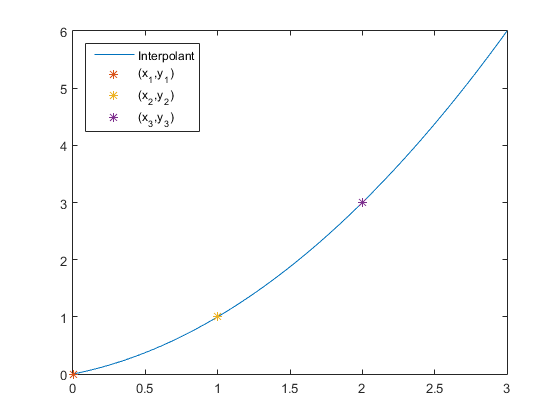
\includegraphics[width=0.5\textwidth]{holmes5_1.png}
				\caption{Graph of $y$ and the data points}
			\end{figure} \

			\item

		\end{enumerate}

\end{enumerate}

\end{document}
